\section{Mis Estudios y Resultados}
En el centro de tu pantalla verás una cuadrícula (grid) con todos tus estudios médicos. Cada tarjeta de estudio te mostrará una fecha y un estatus visual para que sepas en qué fase se encuentra.

Existen tres estados posibles que notarás mediante íconos gráficos:
\begin{itemize}
    \item \textbf{Pendiente de reporte:} Acabas de realizarte el estudio en la clínica, pero los médicos aún no han empezado a revisarlo. La tarjeta estará bloqueada.
    \item \textbf{Estudio en progreso:} Nuestro médico radiólogo está evaluando e interpretando tus imágenes actualmente. El resultado oficial aún no es emitido; por lo tanto, no puedes hacer clic en la tarjeta.
    \item \textbf{Completado:} Tu reporte radiológico se encuentra finalizado y firmado. La tarjeta será brillante y ya puedes hacer clic en ella para ver los detalles de tu expediente.
\end{itemize}

\subsection{Ver Detalle y Descargar PDF}
Para visualizar tu expediente médico final:
\begin{enumerate}
    \item Navega por tu listado de "Mis Estudios" y localiza la tarjeta que diga que está completada.
    \item Haz clic en cualquier parte de dicha tarjeta. El sistema te redireccionará a una vista detallada del dictamen.
    \item En la pantalla, podrás leer directamente el resumen del Radiólogo. La plataforma detallará explícitamente:
    \begin{itemize}
        \item Motivo del estudio clínico.
        \item Hallazgos y mediciones técnicas.
        \item Impresión diagnóstica o conclusiones.
        \item Recomendaciones.
    \end{itemize}
    \item Al inicio del documento, podras ver una previsualización de el estudio digital, al darle clic a esa sección, podras ver ese estudio en grande.
    \begin{figure}
        \centering
        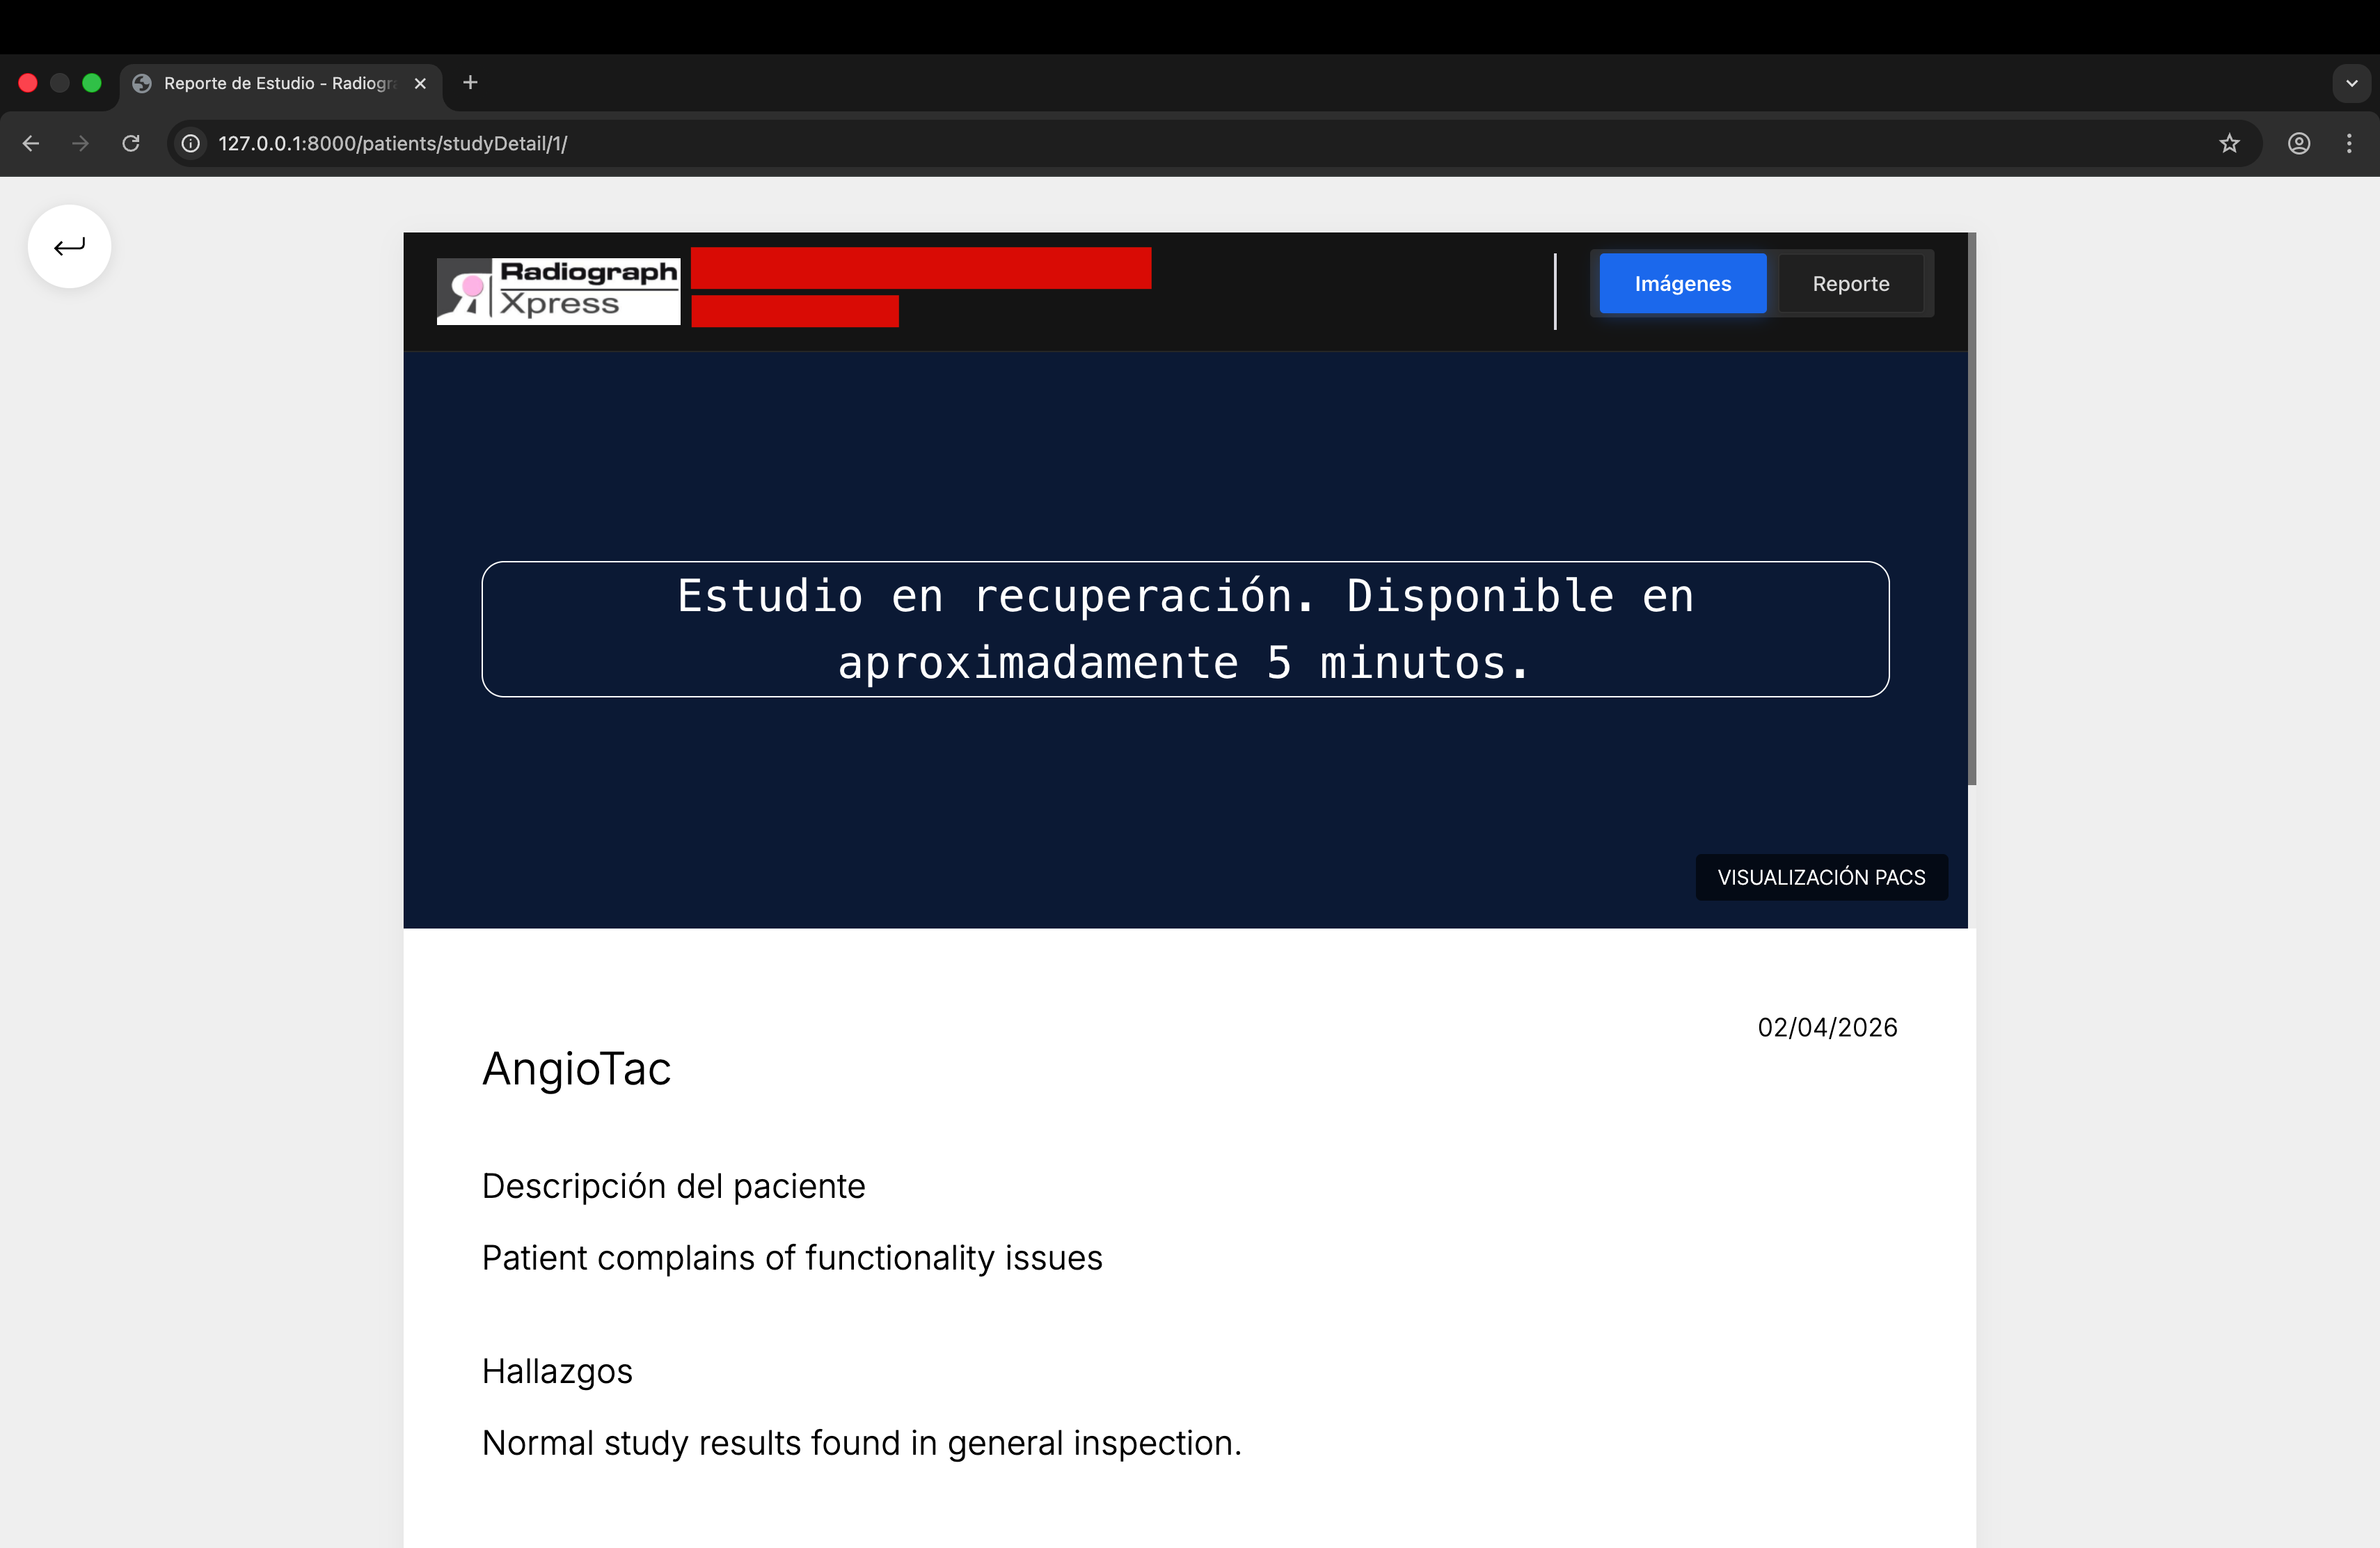
\includegraphics[width=0.5\linewidth]{screenshots/digital_study.png}
        \caption{Ejemplo de visualización del estudio.}
    \end{figure}
    \item Al final del documento virtual, encontrarás la \textbf{Firma Digital} autógrafa del médico especialista en turno avalando que todo está correcto.
    \item Si necesitas entregar estos resultados de manera presencial a tu médico general, localiza el botón rectangular situado en pantalla que dice \textbf{"Descargar reporte PDF"}.
    \item Al presionarlo, RadiographXpress generará de manera instantánea tu reporte estructurado, con sellos y formato institucional, que se descargará en tu computadora/celular listo para imprimirse.
\end{enumerate}
